\documentclass{hcmut-report}
\usepackage{codespace}
\usepackage{graphicx}
\usepackage{hyperref}
\usepackage{float}
\usepackage{amsmath}

\title{Lab 2: Timer Interrupt and LED Scanning}
\coursename{Microcontroller}
\reporttype{Lab Report}
\stuname{Âu Lê Quang Trí - 2453300}

\begin{document}
\coverpage

\tableofcontents
\newpage

\section{Introduction and Timer Interrupt Setup}

\subsection{Principles of LED Scanning (Multiplexing)}
In embedded systems, driving multiple 7-segment displays or LED matrices using individual GPIO pins quickly exhausts the microcontroller's I/O pins. The technique of \textbf{Time-Division Multiplexing (LED scanning)} overcomes this limitation:
\begin{itemize}
    \item All identical segment cathodes (A, B, C, D, E, F, G) from each display are tied together to a common 7-bit bus (PB0--PB6).
    \item The common anode terminal of each display is connected to an independent control switch (such as a PNP transistor or ULN2803 Darlington array), driven by MCU control pins (PA6--PA9).
    \item At any given instant $t$, only one display is powered on with its corresponding segment pattern. By cycling through all displays at a sufficiently high frequency ($f > 30\,\text{Hz}$), the human eye perceives continuous illumination without flicker due to \textbf{Persistence of Vision (POV)}.
\end{itemize}

\subsection{Timer 2 Configuration}
Hardware Timer 2 (TIM2) of the STM32F103C6 is configured to generate periodic interrupts every $10\,\text{ms}$:
\begin{itemize}
    \item \textbf{Clock Source:} Internal High-Speed Clock (HSI) running at $f_{SYS} = 8\,\text{MHz}$.
    \item \textbf{Prescaler (PSC):} Set to $7999$. The timer counting frequency is:
    \begin{equation}
        f_{TIM} = \frac{f_{SYS}}{\text{PSC} + 1} = \frac{8\,\text{MHz}}{7999 + 1} = 1000\,\text{Hz} \quad (T_{tick} = 1\,\text{ms})
    \end{equation}
    \item \textbf{Auto-Reload Register / Period (ARR):} Set to $9$. The counter counts from $0$ up to $9$ (10 counts per overflow event):
    \begin{equation}
        f_{IT} = \frac{f_{TIM}}{\text{ARR} + 1} = \frac{1000\,\text{Hz}}{9 + 1} = 100\,\text{Hz}
    \end{equation}
    \begin{equation}
        T_{IT} = \frac{1}{f_{IT}} = \frac{1}{100\,\text{Hz}} = 10\,\text{ms}
    \end{equation}
    \item \textbf{NVIC Settings:} TIM2 global interrupt is enabled in the NVIC settings.
    \item \textbf{Startup:} Initiated in \texttt{main()} via \texttt{HAL\_TIM\_Base\_Start\_IT(\&htim2)}.
\end{itemize}

\newpage
\section{Exercise 1: Interfacing Two 7-Segment LEDs}

\subsection*{Report 1: Schematic}
The Proteus schematic implementing two common-anode 7-segment displays controlled via PNP transistors (PA6 and PA7) with segment lines connected to PB0--PB6 is illustrated below:

\begin{figure}[H]
    \centering
    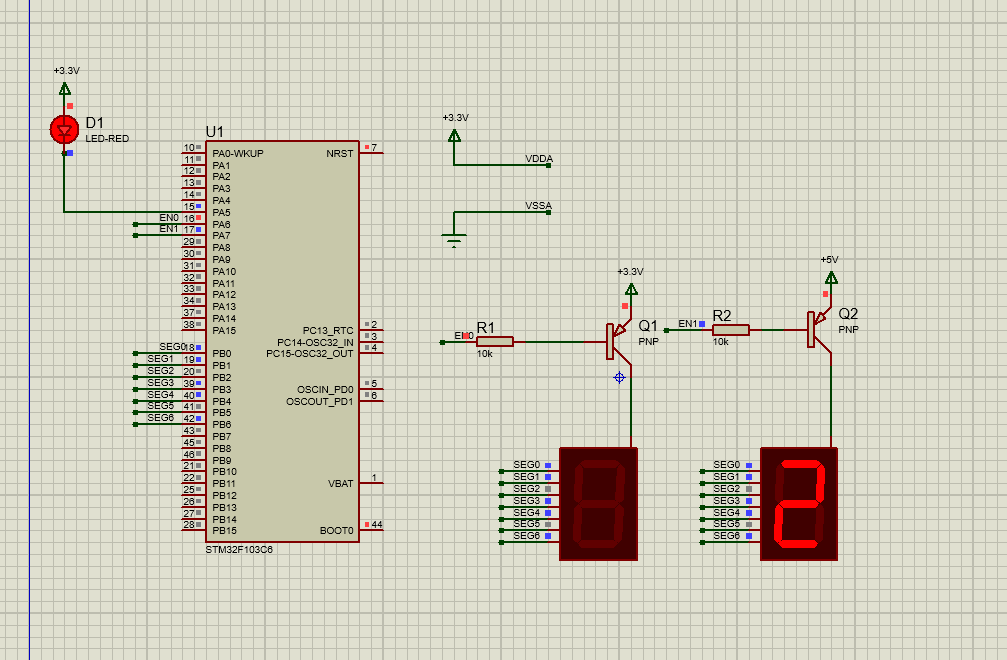
\includegraphics[width=0.85\textwidth]{images/lap2_ex1.png}
    \caption{Proteus simulation schematic for Exercise 1 (Two 7-segment displays)}
    \label{fig:ex1_schematic}
\end{figure}

\subsection*{Report 2: Source Code}
The segment mapping table and the 7-segment decoder function are defined as follows (active-low segments):
\begin{code}{c}
const uint8_t seg_code[10] = {
    0x40, // 0: 0b01000000
    0x79, // 1: 0b01111001
    0x24, // 2: 0b00100100
    0x30, // 3: 0b00110000
    0x19, // 4: 0b00011001
    0x12, // 5: 0b00010010
    0x02, // 6: 0b00000010
    0x78, // 7: 0b01111000
    0x00, // 8: 0b00000000
    0x10  // 9: 0b00010000
};

void display7SEG(int num) {
    if (num < 0 || num > 9) return;
    GPIOB->ODR = seg_code[num];
}
\end{code}

The interrupt service routine \texttt{HAL\_TIM\_PeriodElapsedCallback} toggles between the two displays every $500\,\text{ms}$ ($50 \times 10\,\text{ms}$):
\begin{code}{c}
int counter = 1;   // Initialized to 1 so the first digit displays immediately
int status  = 0;

void HAL_TIM_PeriodElapsedCallback(TIM_HandleTypeDef *htim)
{
    counter--;
    if (counter <= 0) {
        counter = 50;  // 50 x 10ms = 500ms

        // Turn both displays off first to prevent ghosting
        HAL_GPIO_WritePin(GPIOA, GPIO_PIN_6, GPIO_PIN_SET);
        HAL_GPIO_WritePin(GPIOA, GPIO_PIN_7, GPIO_PIN_SET);

        if (status == 0) {
            display7SEG(1);
            HAL_GPIO_WritePin(GPIOA, GPIO_PIN_6, GPIO_PIN_RESET);  // Enable 1st display
            status = 1;
        } else {
            display7SEG(2);
            HAL_GPIO_WritePin(GPIOA, GPIO_PIN_7, GPIO_PIN_RESET);  // Enable 2nd display
            status = 0;
        }
    }
}
\end{code}

\subsection*{Short Question: What is the frequency of the scanning process?}
\textbf{Answer:}
Each 7-segment display is activated for an interval of $T_{\text{display}} = 500\,\text{ms} = 0.5\,\text{s}$.
Because there are $N = 2$ displays in this multiplexed system, a complete cycle scanning both displays requires:
\begin{equation}
    T_{\text{scan}} = N \times T_{\text{display}} = 2 \times 0.5\,\text{s} = 1.0\,\text{s}
\end{equation}
Therefore, the full cycle scanning frequency is:
\begin{equation}
    f_{\text{scan}} = \frac{1}{T_{\text{scan}}} = \frac{1}{1.0\,\text{s}} = 1.0\,\text{Hz}
\end{equation}
(The digit-switching transition rate between successive LEDs is $2\,\text{Hz}$).

\newpage
\section{Exercise 2: Four 7-Segment LEDs with Blinking DOT}

\subsection*{Report 1: Schematic}
The Proteus schematic is extended to four 7-segment displays (enabled by PA6, PA7, PA8, PA9) and two colon DOT LEDs connected to PA4:

\begin{figure}[H]
    \centering
    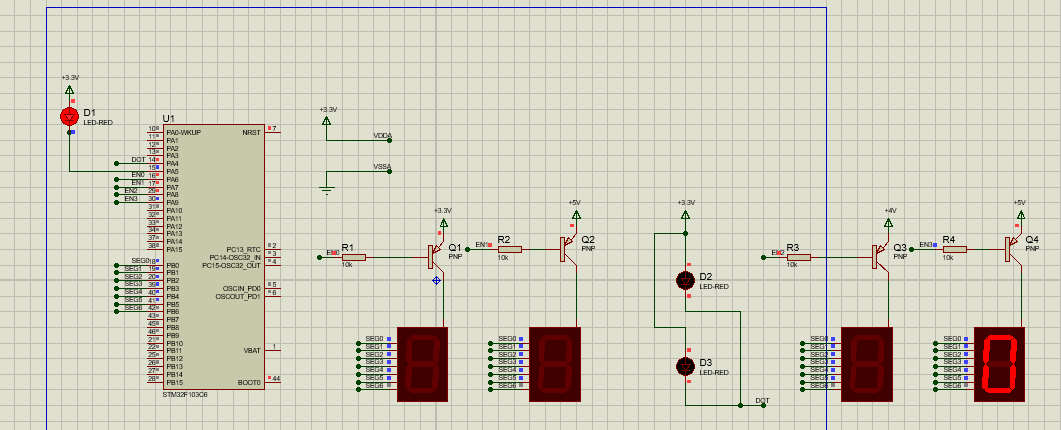
\includegraphics[width=0.88\textwidth]{images/lap2_ex2.png}
    \caption{Proteus schematic for Exercise 2 (Four 7-segment displays and DOT LEDs)}
    \label{fig:ex2_schematic}
\end{figure}

\subsection*{Report 2: Source Code}
The displays show "1", "2", "3", "0" (representing 12:30), switching every $500\,\text{ms}$. The DOT LEDs toggle every second ($100 \times 10\,\text{ms} = 1000\,\text{ms}$):
\begin{code}{c}
int counter = 1;
int status  = 0;
int dot_counter = 100;

void HAL_TIM_PeriodElapsedCallback(TIM_HandleTypeDef *htim)
{
    // Handle DOT LED blinking every 1 second
    dot_counter--;
    if (dot_counter <= 0) {
        dot_counter = 100;
        HAL_GPIO_TogglePin(GPIOA, GPIO_PIN_4);
    }

    // Handle 7-segment scanning every 500ms
    counter--;
    if (counter <= 0) {
        counter = 50;  // 50 x 10ms = 500ms

        // Turn all four displays off first to eliminate ghosting
        HAL_GPIO_WritePin(GPIOA, GPIO_PIN_6, GPIO_PIN_SET);
        HAL_GPIO_WritePin(GPIOA, GPIO_PIN_7, GPIO_PIN_SET);
        HAL_GPIO_WritePin(GPIOA, GPIO_PIN_8, GPIO_PIN_SET);
        HAL_GPIO_WritePin(GPIOA, GPIO_PIN_9, GPIO_PIN_SET);

        switch (status) {
            case 0:
                display7SEG(1);
                HAL_GPIO_WritePin(GPIOA, GPIO_PIN_6, GPIO_PIN_RESET);
                break;
            case 1:
                display7SEG(2);
                HAL_GPIO_WritePin(GPIOA, GPIO_PIN_7, GPIO_PIN_RESET);
                break;
            case 2:
                display7SEG(3);
                HAL_GPIO_WritePin(GPIOA, GPIO_PIN_8, GPIO_PIN_RESET);
                break;
            case 3:
                display7SEG(0);
                HAL_GPIO_WritePin(GPIOA, GPIO_PIN_9, GPIO_PIN_RESET);
                break;
        }
        status = (status + 1) % 4;
    }
}
\end{code}

\subsection*{Short Question: What is the frequency of the scanning process?}
\textbf{Answer:}
Each of the $N = 4$ displays stays active for $T_{\text{display}} = 500\,\text{ms} = 0.5\,\text{s}$. The period required to complete one full scanning round of all 4 displays is:
\begin{equation}
    T_{\text{scan}} = N \times T_{\text{display}} = 4 \times 0.5\,\text{s} = 2.0\,\text{s}
\end{equation}
Consequently, the full-cycle scanning frequency is:
\begin{equation}
    f_{\text{scan}} = \frac{1}{T_{\text{scan}}} = \frac{1}{2.0\,\text{s}} = 0.5\,\text{Hz}
\end{equation}

\newpage
\section{Exercise 3: Implementation of Function \texttt{update7SEG}}

\subsection*{Report 1: Source Code of \texttt{update7SEG}}
To decouple the digit-rendering logic from the timing loop, the buffer \texttt{led\_buffer} and the modular function \texttt{update7SEG(int index)} are implemented:
\begin{code}{c}
const int MAX_LED = 4;
int index_led = 0;
int led_buffer[4] = {1, 2, 3, 4};

void update7SEG(int index) {
    // Turn off all displays to prevent ghosting artifacts
    HAL_GPIO_WritePin(GPIOA, GPIO_PIN_6, GPIO_PIN_SET);
    HAL_GPIO_WritePin(GPIOA, GPIO_PIN_7, GPIO_PIN_SET);
    HAL_GPIO_WritePin(GPIOA, GPIO_PIN_8, GPIO_PIN_SET);
    HAL_GPIO_WritePin(GPIOA, GPIO_PIN_9, GPIO_PIN_SET);

    switch (index) {
        case 0:
            display7SEG(led_buffer[0]);
            HAL_GPIO_WritePin(GPIOA, GPIO_PIN_6, GPIO_PIN_RESET);
            break;
        case 1:
            display7SEG(led_buffer[1]);
            HAL_GPIO_WritePin(GPIOA, GPIO_PIN_7, GPIO_PIN_RESET);
            break;
        case 2:
            display7SEG(led_buffer[2]);
            HAL_GPIO_WritePin(GPIOA, GPIO_PIN_8, GPIO_PIN_RESET);
            break;
        case 3:
            display7SEG(led_buffer[3]);
            HAL_GPIO_WritePin(GPIOA, GPIO_PIN_9, GPIO_PIN_RESET);
            break;
        default:
            break;
    }
}
\end{code}

\subsection*{Report 2: Source Code in \texttt{HAL\_TIM\_PeriodElapsedCallback}}
The callback invokes \texttt{update7SEG} and increments \texttt{index\_led} cyclically:
\begin{code}{c}
int counter = 1;
int dot_counter = 100;

void HAL_TIM_PeriodElapsedCallback(TIM_HandleTypeDef *htim)
{
    dot_counter--;
    if (dot_counter <= 0) {
        dot_counter = 100;
        HAL_GPIO_TogglePin(GPIOA, GPIO_PIN_4);
    }

    counter--;
    if (counter <= 0) {
        counter = 50;  // 50 x 10ms = 500ms
        update7SEG(index_led++);
        if (index_led >= MAX_LED) index_led = 0;
    }
}
\end{code}

\newpage
\section{Exercise 4: Setting the Scanning Frequency to 1 Hz}

\subsection*{Report 1: Source Code in \texttt{HAL\_TIM\_PeriodElapsedCallback}}
To achieve an overall scanning frequency of $f_{\text{scan}} = 1\,\text{Hz}$ across the $4$ displays:
\begin{equation}
    T_{\text{scan}} = \frac{1}{f_{\text{scan}}} = 1.0\,\text{s} = 1000\,\text{ms}
\end{equation}
The time allocation for each individual display must therefore be:
\begin{equation}
    T_{\text{per\_LED}} = \frac{T_{\text{scan}}}{4} = \frac{1000\,\text{ms}}{4} = 250\,\text{ms}
\end{equation}
With the hardware timer tick period of $10\,\text{ms}$, the software counter must be reloaded with:
\begin{equation}
    \text{counter} = \frac{250\,\text{ms}}{10\,\text{ms}} = 25
\end{equation}

The implemented interrupt service routine is:
\begin{code}{c}
int counter = 1;
int dot_counter = 100;

void HAL_TIM_PeriodElapsedCallback(TIM_HandleTypeDef *htim)
{
    // DOT LED continues toggling every second (100 x 10ms = 1000ms)
    dot_counter--;
    if (dot_counter <= 0) {
        dot_counter = 100;
        HAL_GPIO_TogglePin(GPIOA, GPIO_PIN_4);
    }

    // 4-digit display scanning at 1Hz (250ms per digit)
    counter--;
    if (counter <= 0) {
        counter = 25;  // 25 x 10ms = 250ms -> 4 x 250ms = 1000ms = 1s (1Hz)
        update7SEG(index_led++);
        if (index_led >= MAX_LED) index_led = 0;
    }
}
\end{code}

\newpage
\section{Exercise 5: Digital Clock with Hour and Minute Buffer}

\subsection*{Report 1: Source Code in \texttt{updateClockBuffer}}
To implement a digital clock, the time variables \texttt{hour}, \texttt{minute}, and \texttt{second} are maintained. The function \texttt{updateClockBuffer} extracts the tens and units digits of the current time and populates the 4-element array \texttt{led\_buffer}:
\begin{code}{c}
int hour = 15, minute = 8, second = 50;

void updateClockBuffer(void) {
    led_buffer[0] = hour / 10;    // Tens of the hour
    led_buffer[1] = hour % 10;    // Units of the hour
    led_buffer[2] = minute / 10;  // Tens of the minute
    led_buffer[3] = minute % 10;  // Units of the minute
}
\end{code}

In the \texttt{main()} loop, the clock advances every second using \texttt{HAL\_Delay(1000)}:
\begin{code}{c}
while (1)
{
    second++;
    if (second >= 60) {
        second = 0;
        minute++;
    }
    if (minute >= 60) {
        minute = 0;
        hour++;
    }
    if (hour >= 24) {
        hour = 0;
    }
    updateClockBuffer();
    HAL_Delay(1000);
}
\end{code}

\newpage
\section{Exercise 6: Software Timer Implementation and Analysis}

\subsection{Software Timer Concept}
Relying on blocking functions like \texttt{HAL\_Delay()} stalls the processor and wastes CPU cycles. Furthermore, placing excessive computation inside the interrupt handler can cause interrupt latency and nested interrupt crashes.
A \textbf{software timer} maintains an integer counter decremented in the $10\,\text{ms}$ hardware timer ISR. When the counter reaches zero, a software flag is raised, signaling the background \texttt{main()} loop to execute the scheduled task non-blockingly:
\begin{code}{c}
#define TIMER_CYCLE 10  // ms per timer interrupt tick

int timer0_counter = 0;
volatile int timer0_flag = 0;

void setTimer0(int duration) {
    timer0_counter = duration / TIMER_CYCLE;
    timer0_flag = 0;
}

void timer_run(void) {
    if (timer0_counter > 0) {
        timer0_counter--;
        if (timer0_counter == 0) timer0_flag = 1;
    }
}
\end{code}

The test code in \texttt{main()}:
\begin{code}{c}
setTimer0(1000);
while (1) {
    if (timer0_flag == 1) {
        HAL_GPIO_TogglePin(LED_RED_GPIO_Port, LED_RED_Pin);
        setTimer0(2000);
    }
}
\end{code}

\subsection*{Report 1: Analysis if line 1 (\texttt{setTimer0(1000)}) is missed}
\textbf{Question:} If in line 1 of the code above is missed, what happens after that and why?

\textbf{Answer:}
\begin{itemize}
    \item \textbf{Observation:} The LED will never toggle and will remain permanently in its initial state.
    \item \textbf{Cause:} \texttt{timer0\_counter} is initialized to $0$, and \texttt{timer0\_flag} is initialized to $0$. When hardware interrupts occur every $10\,\text{ms}$, the ISR invokes \texttt{timer\_run()}. Inside \texttt{timer\_run()}, the condition \texttt{if (timer0\_counter > 0)} evaluates to \textbf{false} ($0 > 0$ is false). Therefore, \texttt{timer0\_counter} is never decremented, and the assignment \texttt{timer0\_flag = 1} is never reached. Consequently, in \texttt{main()}, the polling condition \texttt{if (timer0\_flag == 1)} will never become true, stalling the toggle mechanism completely.
\end{itemize}

\subsection*{Report 2: Analysis if line 1 is changed to \texttt{setTimer0(1)}}
\textbf{Question:} If in line 1 of the code above is changed to \texttt{setTimer0(1)}, what happens after that and why?

\textbf{Answer:}
\begin{itemize}
    \item \textbf{Observation:} The LED will also never toggle and remains stuck in its initial state.
    \item \textbf{Cause:} In C programming, integer division truncates fractions toward zero:
    \begin{equation}
        \text{timer0\_counter} = \frac{\text{duration}}{\text{TIMER\_CYCLE}} = \frac{1}{10} = 0
    \end{equation}
    Because \texttt{timer0\_counter} evaluates to $0$ and \texttt{timer0\_flag} is cleared to $0$, the subsequent interrupt executions in \texttt{timer\_run()} encounter $\text{timer0\_counter} = 0$. Since $0$ is not strictly greater than $0$, the counter is never decremented and \texttt{timer0\_flag} is never set to $1$. The condition in the \texttt{while(1)} loop is never triggered.
\end{itemize}

\subsection*{Report 3: Analysis if line 1 is changed to \texttt{setTimer0(10)}}
\textbf{Question:} If in line 1 of the code above is changed to \texttt{setTimer0(10)}, what is changed compared to the first two questions and why?

\textbf{Answer:}
\begin{itemize}
    \item \textbf{Observation:} The LED successfully toggles! Specifically, the first toggle occurs almost immediately (exactly $10\,\text{ms}$ after startup), after which the LED toggles periodically every $2000\,\text{ms}$ ($2$ seconds).
    \item \textbf{Cause:} With $\text{duration} = 10\,\text{ms}$, the integer division yields:
    \begin{equation}
        \text{timer0\_counter} = \frac{10}{10} = 1
    \end{equation}
    At the very first hardware timer interrupt (after $10\,\text{ms}$), \texttt{timer\_run()} decrements \texttt{timer0\_counter} from $1$ to $0$. Since it reaches $0$, \texttt{timer0\_flag} is set to $1$. In the \texttt{main()} loop, \texttt{if (timer0\_flag == 1)} is satisfied: the LED toggles at $t = 10\,\text{ms}$, and the software timer is immediately rearmed with \texttt{setTimer0(2000)} (\texttt{timer0\_counter} $= 2000 / 10 = 200$). From then on, the LED blinks reliably with a half-period of $2\,\text{s}$.
\end{itemize}

\newpage
\section{Exercise 7: Upgrading Digital Clock with Software Timer}

\subsection*{Report 1: Source Code in the \texttt{while (1)} Loop}
The blocking delay \texttt{HAL\_Delay(1000)} is replaced by calling \texttt{setTimer0(1000)} and checking \texttt{timer0\_flag}. In addition, the DOT LED toggle is moved to \texttt{main()}:
\begin{code}{c}
/* USER CODE BEGIN 2 */
HAL_TIM_Base_Start_IT(&htim2);
updateClockBuffer();
setTimer0(1000);
/* USER CODE END 2 */

while (1)
{
    /* USER CODE BEGIN 3 */
    if (timer0_flag == 1) {
        setTimer0(1000);  // Rearm software timer for the next 1 second interval
        second++;
        if (second >= 60) {
            second = 0;
            minute++;
        }
        if (minute >= 60) {
            minute = 0;
            hour++;
        }
        if (hour >= 24) {
            hour = 0;
        }
        updateClockBuffer();
        HAL_GPIO_TogglePin(GPIOA, GPIO_PIN_4);  // Toggle colon DOT in main()
    }
}
\end{code}

The timer ISR handles decrementing the timer counter and scanning the displays:
\begin{code}{c}
void HAL_TIM_PeriodElapsedCallback(TIM_HandleTypeDef *htim)
{
    timer_run();
    counter--;
    if (counter <= 0) {
        counter = 25;  // 250ms scanning rate per digit
        update7SEG(index_led++);
        if (index_led >= MAX_LED) index_led = 0;
    }
}
\end{code}

\newpage
\section{Exercise 8: Moving Display Scanning to \texttt{main()}}

\subsection*{Report 1: Source Code in \texttt{main()} and Software Timer System}
To optimize interrupt performance, all display updating is moved out of the ISR into \texttt{main()}. The timer interrupt is dedicated solely to ticking software timers. An array-based multi-timer architecture is implemented:
\begin{code}{c}
#define TIMER_CYCLE  10  // 10ms tick
#define NO_OF_TIMERS 4

#define TIMER_SECOND 0   // Clock tick & DOT (1000ms)
#define TIMER_SCAN7  1   // 7-segment multiplexing (250ms)
#define TIMER_MATRIX 2   // LED Matrix scanning
#define TIMER_SHIFT  3   // Matrix animation

int timer_counter[NO_OF_TIMERS];
volatile int timer_flag[NO_OF_TIMERS];

void setTimer(int index, int duration) {
    timer_counter[index] = duration / TIMER_CYCLE;
    timer_flag[index] = 0;
}

void timer_run(void) {
    for (int i = 0; i < NO_OF_TIMERS; i++) {
        if (timer_counter[i] > 0) {
            timer_counter[i]--;
            if (timer_counter[i] == 0) timer_flag[i] = 1;
        }
    }
}
\end{code}

The ISR is now extremely lean ($O(1)$ operations with minimal register usage):
\begin{code}{c}
void HAL_TIM_PeriodElapsedCallback(TIM_HandleTypeDef *htim)
{
    timer_run();
}
\end{code}

The complete non-blocking background loop in \texttt{main()}:
\begin{code}{c}
/* USER CODE BEGIN 2 */
HAL_TIM_Base_Start_IT(&htim2);
updateClockBuffer();
setTimer(TIMER_SECOND, 1000);
setTimer(TIMER_SCAN7, 250);
/* USER CODE END 2 */

while (1)
{
    // Task 1: 1-second clock increment and DOT blinking
    if (timer_flag[TIMER_SECOND] == 1) {
        setTimer(TIMER_SECOND, 1000);
        second++;
        if (second >= 60) {
            second = 0;
            minute++;
        }
        if (minute >= 60) {
            minute = 0;
            hour++;
        }
        if (hour >= 24) {
            hour = 0;
        }
        updateClockBuffer();
        HAL_GPIO_TogglePin(GPIOA, GPIO_PIN_4);
    }

    // Task 2: 7-segment display scanning every 250ms
    if (timer_flag[TIMER_SCAN7] == 1) {
        setTimer(TIMER_SCAN7, 250);
        update7SEG(index_led++);
        if (index_led >= MAX_LED) index_led = 0;
    }
}
\end{code}

\newpage
\section{Exercise 9: 8x8 LED Matrix Display}

\subsection*{Report 1: Schematic}
The Proteus schematic incorporates the \texttt{MATRIX-8X8-RED} and a \texttt{ULN2803} Darlington transistor array. The row pins (ROW0--ROW7) are wired to PB8--PB15, while the column enable lines (ENM0--ENM7) are wired to GPIOA pins:

\begin{figure}[H]
    \centering
    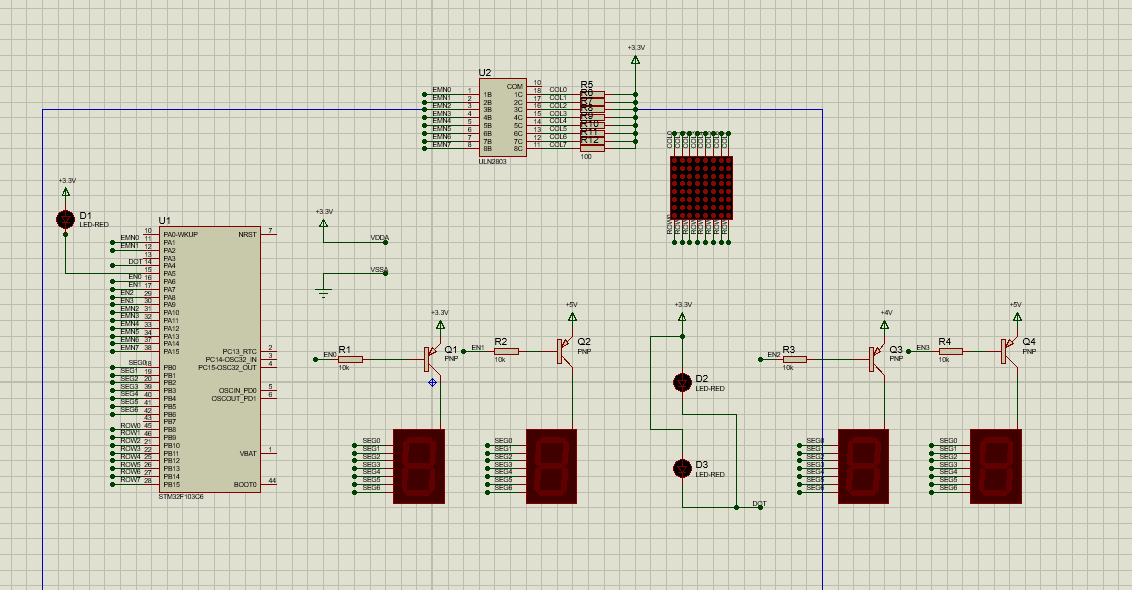
\includegraphics[width=0.92\textwidth]{images/lap2_ex9.png}
    \caption{Proteus schematic for Exercise 9 (8x8 LED Matrix with ULN2803 driver)}
    \label{fig:ex9_schematic}
\end{figure}

\subsection*{Report 2: Source Code of \texttt{updateLEDMatrix}}
To display the character "A", the bitmap buffer is defined per column (with bit 0 corresponding to ROW0 at the top). Because the 7-segment displays use PB0--PB6, the 7-segment display function is refined to modify only bits 0--6 of \texttt{GPIOB->ODR}, preserving the matrix row data on PB8--PB15:
\begin{code}{c}
void display7SEG(int num) {
    if (num < 0 || num > 9) return;
    GPIOB->ODR = (GPIOB->ODR & ~0x007F) | seg_code[num];
}

const int MAX_LED_MATRIX = 8;
int index_led_matrix = 0;

// Column bitmap for character 'A' (columns 0 to 7)
uint8_t matrix_buffer[8] = {0xFC, 0xFE, 0x13, 0x11, 0x11, 0x13, 0xFE, 0xFC};

const uint16_t enm_pin[8] = {
    GPIO_PIN_1,  GPIO_PIN_2,  GPIO_PIN_10, GPIO_PIN_11,
    GPIO_PIN_12, GPIO_PIN_13, GPIO_PIN_14, GPIO_PIN_15
};

#define ENM_ON     GPIO_PIN_RESET  // ULN2803 inverts input: LOW on MCU enables driver
#define ENM_OFF    GPIO_PIN_SET
#define ROW_INVERT 1

static void matrixShow(int col) {
    // 1. Turn off all columns to avoid ghosting
    for (int i = 0; i < 8; i++) {
        HAL_GPIO_WritePin(GPIOA, enm_pin[i], ENM_OFF);
    }
    // 2. Output row pattern onto PB8..PB15
    uint8_t data = matrix_buffer[col];
    if (ROW_INVERT) data = (uint8_t)~data;
    GPIOB->ODR = (GPIOB->ODR & ~0xFF00) | ((uint32_t)data << 8);

    // 3. Enable the active column
    HAL_GPIO_WritePin(GPIOA, enm_pin[col], ENM_ON);
}

void updateLEDMatrix(int index) {
    switch (index) {
        case 0: matrixShow(0); break;
        case 1: matrixShow(1); break;
        case 2: matrixShow(2); break;
        case 3: matrixShow(3); break;
        case 4: matrixShow(4); break;
        case 5: matrixShow(5); break;
        case 6: matrixShow(6); break;
        case 7: matrixShow(7); break;
        default: break;
    }
}
\end{code}

In \texttt{main()}, the matrix is scanned every $10\,\text{ms}$ (\texttt{setTimer(TIMER\_MATRIX, 10)}):
\begin{code}{c}
if (timer_flag[TIMER_MATRIX] == 1) {
    setTimer(TIMER_MATRIX, 10);
    updateLEDMatrix(index_led_matrix++);
    if (index_led_matrix >= MAX_LED_MATRIX) index_led_matrix = 0;
}
\end{code}

\newpage
\section{Exercise 10: LED Matrix Animation (Horizontal Scrolling)}

\subsection*{Report 1: Animation Solution Description and Source Code}
\textbf{Algorithm Description:}
To create a smooth left-scrolling animation of character "A":
\begin{enumerate}
    \item A circular column shift buffer is implemented in function \texttt{shiftLeft()}.
    \item Every column $i$ ($0 \le i < 7$) copies the bitmap data of its right neighbor $i + 1$:
    \begin{equation}
        \text{matrix\_buffer}[i] = \text{matrix\_buffer}[i+1]
    \end{equation}
    \item The leftmost column (\texttt{matrix\_buffer[0]}), which shifts out of the visible screen, wraps around to the rightmost column (\texttt{matrix\_buffer[7]}).
    \item \textbf{Decoupled Timing:} The column multiplexing runs rapidly at $10\,\text{ms}$ per column (yielding a full matrix refresh rate of $f_{\text{refresh}} = \frac{1}{8 \times 10\,\text{ms}} = 12.5\,\text{Hz}$), ensuring crisp POV illumination. The scrolling animation is driven by a independent software timer (\texttt{TIMER\_SHIFT}) set to $200\,\text{ms}$ per step, generating a fluid shift motion across the matrix.
\end{enumerate}

The implementation of \texttt{shiftLeft()} and the main scheduling logic:
\begin{code}{c}
void shiftLeft(void) {
    uint8_t first = matrix_buffer[0];
    for (int i = 0; i < MAX_LED_MATRIX - 1; i++) {
        matrix_buffer[i] = matrix_buffer[i + 1];  // Shift left
    }
    matrix_buffer[MAX_LED_MATRIX - 1] = first;    // Wrap around to rightmost column
}
\end{code}

The complete scheduling loop in \texttt{main()}:
\begin{code}{c}
/* USER CODE BEGIN 2 */
HAL_TIM_Base_Start_IT(&htim2);
updateClockBuffer();
setTimer(TIMER_SECOND, 1000);
setTimer(TIMER_SCAN7, 250);
setTimer(TIMER_MATRIX, 10);
setTimer(TIMER_SHIFT, 200);
/* USER CODE END 2 */

while (1)
{
    // 1. Clock increment and DOT toggle (1000ms)
    if (timer_flag[TIMER_SECOND] == 1) {
        setTimer(TIMER_SECOND, 1000);
        second++;
        if (second >= 60) {
            second = 0;
            minute++;
        }
        if (minute >= 60) {
            minute = 0;
            hour++;
        }
        if (hour >= 24) {
            hour = 0;
        }
        updateClockBuffer();
        HAL_GPIO_TogglePin(GPIOA, GPIO_PIN_4);
    }

    // 2. 7-segment scanning (250ms)
    if (timer_flag[TIMER_SCAN7] == 1) {
        setTimer(TIMER_SCAN7, 250);
        update7SEG(index_led++);
        if (index_led >= MAX_LED) index_led = 0;
    }

    // 3. LED matrix column scanning (10ms)
    if (timer_flag[TIMER_MATRIX] == 1) {
        setTimer(TIMER_MATRIX, 10);
        updateLEDMatrix(index_led_matrix++);
        if (index_led_matrix >= MAX_LED_MATRIX) index_led_matrix = 0;
    }

    // 4. Matrix animation shift left (200ms)
    if (timer_flag[TIMER_SHIFT] == 1) {
        setTimer(TIMER_SHIFT, 200);
        shiftLeft();
    }
}
\end{code}

\section{Source Code and Repository}
All STM32CubeIDE project files, C source code, Proteus simulation circuits, and \LaTeX{} report files are maintained at our GitHub repository:
\begin{center}
    \url{https://github.com/aulequangtri/microprocessor_lab}
\end{center}

\end{document}
